\documentclass[11pt]{beamer}
\usetheme{Berlin}
\usepackage[utf8]{inputenc}
\usepackage{amsmath}
\usepackage{amsfonts}
\usepackage{amssymb}
\usepackage{algorithm2e}
\usepackage{stmaryrd}
\usepackage[utf8]{inputenc}
\usepackage{graphicx}
\usepackage{caption}
\usepackage{subcaption}
\usepackage{verbatim}
\usepackage{tikz}


\defbeamertemplate*{footline}{shadow theme}
{%
  \leavevmode%
  \hbox{\begin{beamercolorbox}[wd=.5\paperwidth,ht=2.5ex,dp=1.125ex,leftskip=.3cm plus1fil,rightskip=.3cm]{author in head/foot}%
    \usebeamerfont{author in head/foot}\insertframenumber\,/\,\inserttotalframenumber\hfill\insertshortauthor
  \end{beamercolorbox}%
  \begin{beamercolorbox}[wd=.5\paperwidth,ht=2.5ex,dp=1.125ex,leftskip=.3cm,rightskip=.3cm plus1fil]{title in head/foot}%
    \usebeamerfont{title in head/foot}\insertshorttitle%
  \end{beamercolorbox}}%
  \vskip0pt%
}
\DeclareMathOperator*{\argmax}{arg\,max}
\DeclareMathOperator*{\argmin}{arg\,min}
\author{Louis Cohen \& Adele Mortier}
\title{Smallworld}
%\setbeamercovered{transparent} 
%\setbeamertemplate{navigation symbols}{}
%\logo{} 
\institute{MPRI 2017} 
\date{February 25, 2018} 
%\subject{} 
\begin{document}

\begin{frame}
\titlepage
\end{frame}

\begin{frame}
\tableofcontents
\end{frame}

\section{Introduction}

\begin{frame}[fragile]{Introduction}
	
	Mimic the people's behavior in a big city :
	\begin{alertblock}{Problems}
	\begin{itemize}
		\item Everyday life planning ?
		\item Use of the transportation network ?
	\end{itemize}
	\end{alertblock}
	Tools we used :
	\begin{figure}
		\centering
		\begin{subfigure}{.24\textwidth}
			\centering
			
\includegraphics[width=.5\linewidth]{images/python.png}
		\end{subfigure}%
		\begin{subfigure}{.24\textwidth}
			\centering
			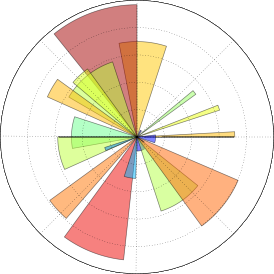
\includegraphics[width=.5\linewidth]{images/matplotlib.png}
		\end{subfigure}%
		\begin{subfigure}{.24\textwidth}
			\centering
			
\includegraphics[width=.5\linewidth]{images/sympy.png}
		\end{subfigure}%
		\begin{subfigure}{.24\textwidth}
			\centering
			
\includegraphics[width=.5\linewidth]{images/sklearn.png}
		\end{subfigure}
	\end{figure}
\end{frame}

\section{Transportation network}
\subsection{Topology}
\begin{frame}{Topology -- main steps}
	Subway network $\sim$ Parisian ``metro''.
	\begin{block}{Steps}
		\begin{enumerate}
			\item \textbf{Terminals} : line segments.
			\item \textbf{Intersections} : point clustering.
			\item \textbf{Stations} : points at regular intervals. 
			\item \textbf{Hubs} : stations crossed by many lines.
			\item \textbf{Fast lines} : connect hubs together.
		\end{enumerate}
	\end{block}
\end{frame}

\begin{frame}{Topology -- illustrations}
	\begin{figure}
		\centering
		\captionsetup{justification=centering}
			
		\begin{subfigure}[t]{.3\textwidth}
			\centering
			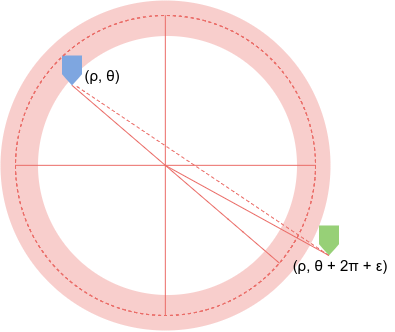
\includegraphics[width=0.8\linewidth]{images/create_line.png}
			\caption{Terminals : originate in the suburbs, go through the center}
		\end{subfigure}\qquad%
		\begin{subfigure}[t]{.3\textwidth}
			\centering
			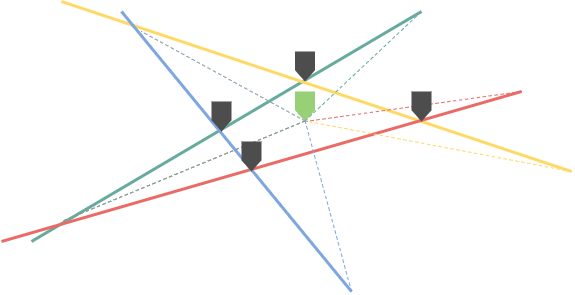
\includegraphics[width=\linewidth]{images/glue_intersections.png}
			\caption{Intersections : move close intersections to their centroid}
		\end{subfigure}\qquad%
		\begin{subfigure}[t]{.3\textwidth}
			\centering
			
\includegraphics[width=\linewidth]{images/station_creation.png}
			\caption{Stations : sample the line and add noise}
		\end{subfigure}
	\end{figure}
\end{frame}

\begin{frame}{Topology -- results}
	\begin{figure}
		\centering
		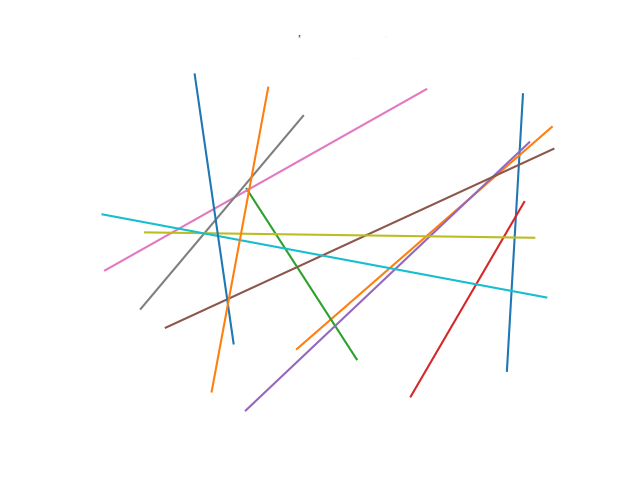
\includegraphics[width=0.7\linewidth]{images/net_1.png}
		\caption{Terminals generation -- subway lines are simple segments}
	\end{figure}
\end{frame}
\begin{frame}{Topology -- results}
	\begin{figure}
		\centering
		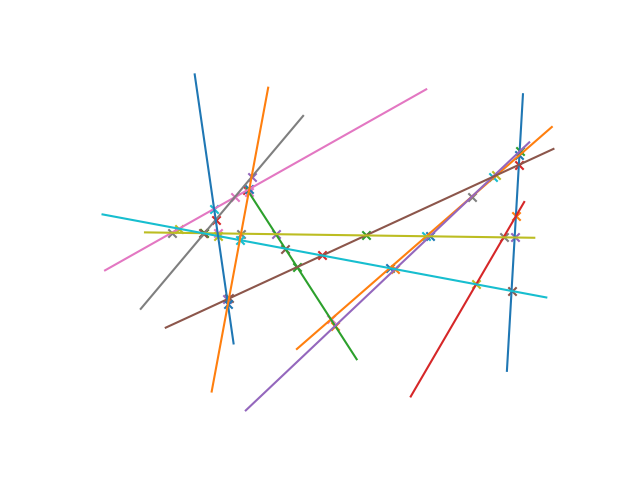
\includegraphics[width=0.7\linewidth]{images/net_2.png}
		\caption{Intersection resolution -- find where the lines cross using SymPy}
	\end{figure}
\end{frame}
\begin{frame}{Topology -- results}
	\begin{figure}
		\centering
		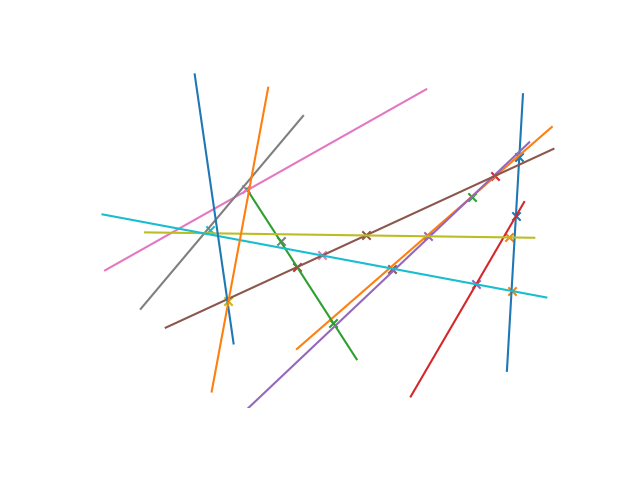
\includegraphics[width=0.7\linewidth]{images/net_3.png}
		\caption{Intersection gluing -- merge close intersections using a clustering algorithm (DBSCAN)}
	\end{figure}
\end{frame}
\begin{frame}{Topology -- results}
	\begin{figure}
		\centering
		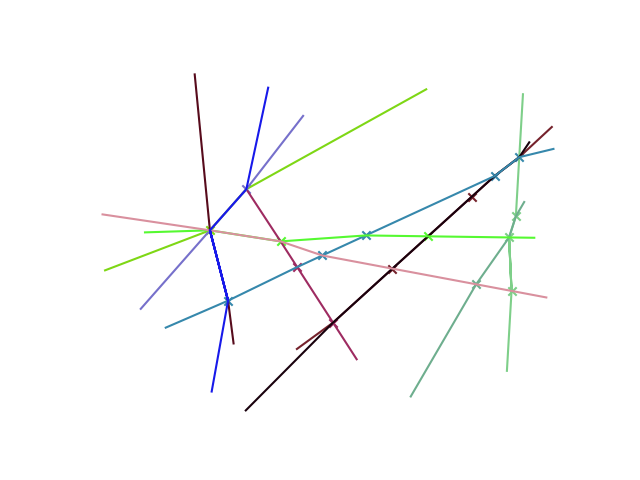
\includegraphics[width=0.7\linewidth]{images/net_4.png}
		\caption{Line bending -- bend te lines such that they cross glued intersections}
	\end{figure}
\end{frame}
\begin{frame}{Topology -- results}
	\begin{figure}
		\centering
		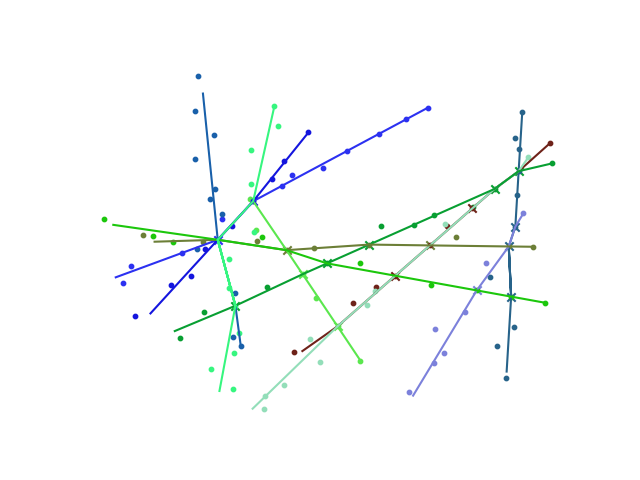
\includegraphics[width=0.7\linewidth]{images/net_5.png}
		\caption{Stations -- put stations at regular intervals plus a little noise}
	\end{figure}
\end{frame}
\begin{frame}{Topology -- results}
	\begin{figure}
		\centering
		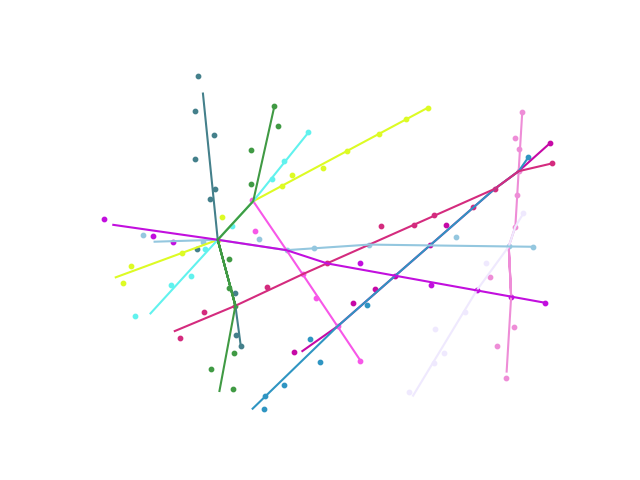
\includegraphics[width=0.7\linewidth]{images/net_6.png}
		\caption{Stations gluing -- merge close intersections with DBSCAN again}
	\end{figure}
\end{frame}
\begin{frame}{Topology -- results}
	\begin{figure}
		\centering
		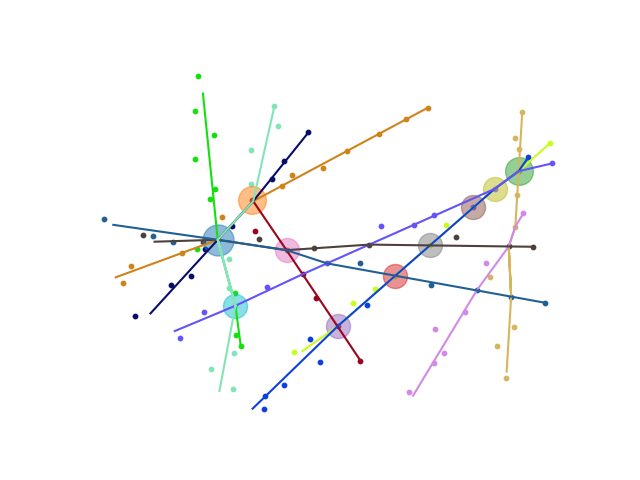
\includegraphics[width=0.7\linewidth]{images/net_7.png}
		\caption{Hubs -- find stations with many lines crossing them and generate fast lines}
	\end{figure}
\end{frame}


\subsection{Toponymy}
\begin{frame}{Toponymy -- main steps}
	 ``Realistic'' stations' names, \textit{e.g.} ``Place Edith Piaf'', ``Rue de la Chine'' or ``Saint Marcel''...
	\begin{block}{Steps}
		\begin{enumerate}
			\item \textbf{Data collection} : collect from databases or manually.
			\item \textbf{Combine elements together} : link words (``Place de la/le'', ``Saint(e)'', ``-''...).
			\item \textbf{Do some tricks} : avoid things like ``Place d'Arc'' or ``Avenue de Maupassant''... 
		\end{enumerate}
	\end{block}
	\textbf{``Best-of''} : ``Avenue Johnny Hallyday'', ``Gare Nabilla'', ``Rue du Swaziland''...
\end{frame}

\begin{frame}
		\begin{figure}
			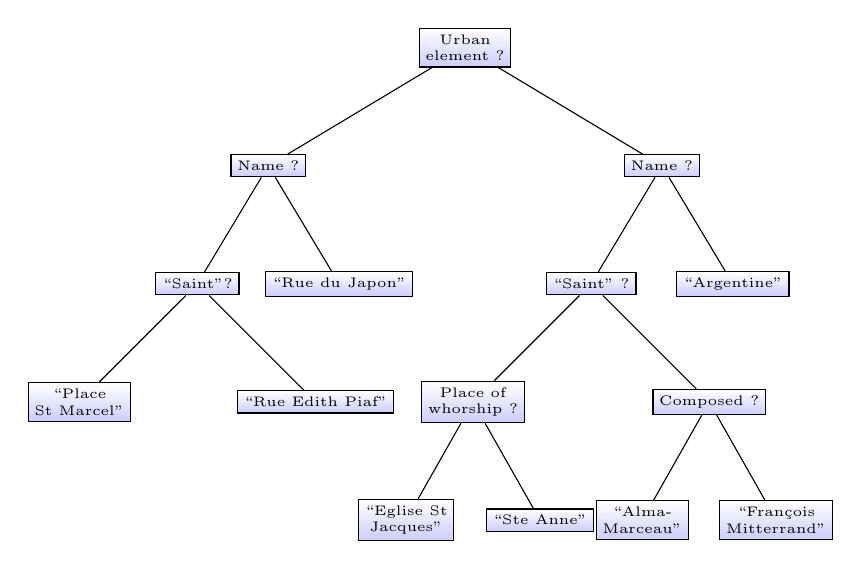
\begin{tikzpicture}[
		level 1/.style={sibling distance=50mm},
		level 2/.style={sibling distance=18mm},
		level 3/.style={sibling distance=30mm},
		level 4/.style={sibling distance=17mm},
		level 5/.style={sibling distance=10mm},
		every node/.style = {shape=rectangle,
			draw, align=center,
			top color=white, bottom color=blue!20}]
		\tiny
		\node {Urban \\ element ?}
		child { node {Name ?}
			child { node {``Saint''?}
				child { node {``Place \\ St Marcel''}}
				child { node {``Rue Edith Piaf''}}}
			child { node {``Rue du Japon''} } }
		child { node {Name ?} 
			child { node {``Saint'' ?}
			child { node {Place of\\whorship ?}
				child { node {``Eglise St\\ Jacques''} }
				child { node {``Ste Anne''} }}
			child { node {Composed ?}
				child { node {``Alma-\\Marceau''}}
				child { node {``François\\ Mitterrand''}}
			} 
			}
		child { node {``Argentine''}}}
;
		\end{tikzpicture}
		\caption{Simplified binary tree for name generation}
		\end{figure}
\end{frame}

\subsection{Schedule}
\begin{frame}{Schedule -- main steps}
	Station schedule $Rightarrow$ point to point travel times.
	\begin{block}{Steps}
		\begin{enumerate}
		\item Travel times between stations $\propto$ line speed, distance.
		\item Departure times from terminals $\propto$ moment of the day.
		\item Propagate the departure times along the line using the values computed at first step.
		\item Use the schedule to compute a shortest path that is sensitive to de day/hour of departure (\textbf{not implemented})
		\end{enumerate}
	\end{block} 
\end{frame}
\begin{frame}{Schedule --  illustration}
	\begin{figure}
		\centering
		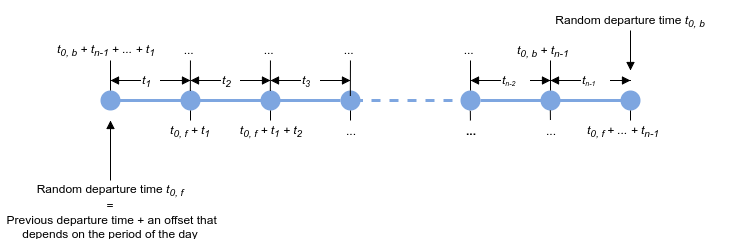
\includegraphics[width=\linewidth]{images/schedule.png}
		\caption{Computation of a line of the schedule for one subway line}
	\end{figure}
\end{frame}0
\section{Generating persons deplacement}
\subsection{General Idea}

\begin{frame}{}

\begin{block}{Key ideas}
\begin{itemize}
\item Families
\item Work
\item Activities
\item Home
\item Deplacement between those points !
\end{itemize}
\end{block}
\end{frame}


\begin{frame}{Localisation ideas}
Center : working \\
Subburbs : housing \\
(all probabilistic)\\
\includegraphics[scale=.5]{subburb}


\end{frame}
\subsection{A person}

\begin{frame}{A person}
\begin{itemize}
\item Id
\item Age
\item Work type and informations
\item Work location
\item Home location
\item Family
\item Typical activities
\item Planning
\end{itemize}
\end{frame}


\begin{frame}{Persons models}
\begin{block}{How to differentiate}
Typical activities\\
Days worked \\
Work position
\end{block}

\begin{alertblock}{Persons type}
\begin{itemize}
\item Students : work near home location, ludic activities, student weak
\item White collar : working in center, groceries, different work shedule
\item Unenmployed : 
\end{itemize}

\end{alertblock}


\end{frame}


\begin{frame}{Generating families}
\begin{itemize}
\item one or two parents
\item several childs
\end{itemize}
\end{frame}
\end{document}

